\setAuthor{Jaan Kalda}
\setRound{piirkonnavoor}
\setYear{2008}
\setNumber{G 2}
\setDifficulty{3}
\setTopic{Kinemaatika}

\prob{Autod}
Juuresolev joonis on tehtud kõrgelt otse alla pildistatud foto põhjal, millel on jäädvustatud kaks autot (tähistatud punktidega $A$ ja $B$), mis lähenevad ristmikule jäävate kiirustega $v_A = \SI{40}{km/h}$ ja $v_B = \SI{60}{km/h}$. Kasutades joonist ja sellel antud mõõtkava, leidke autode edasisel liikumisel nende vaheline minimaalne kaugus.

\begin{center}
	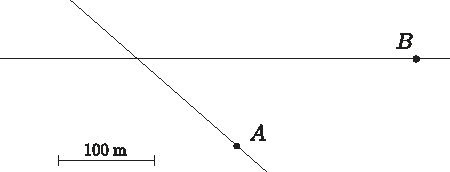
\includegraphics[width=0.9\linewidth]{2008-v2g-02-yl}
\end{center}

\hint
Ülesannet on mugavam vaadelda emma-kumma autoga seotud taustsüsteemis.

\solu
Kanname joonisele autode $A$ ja $B$ kiirusvektorid suvalises mõõtkavas (st vektorite moodulid suhtuvad nagu 40:60). Leiame nende vektorite vahe, see on autode suhteline kiirus. Tõmmates ühe auto juurest selle vektori sihilise sirge leiame tema trajektoori teise autoga seotud süsteemis. Teise auto kaugus sellest sirgest annabki vastuse. Mõõtkava arvestamine ja mõistlik numbriline tulemus annab \SI{60}{m}.
\begin{center}
	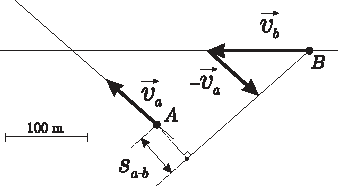
\includegraphics[width=0.7\linewidth]{2008-v2g-02-lah}
\end{center}
\probend